\documentclass[14pt,aspectratio=169]{beamer}
\usetheme{default}
\setbeamertemplate{navigation symbols}{}

\usepackage{fontspec}
\IfFontExistsTF{Times New Roman}{%
  \setmainfont{Times New Roman}%
}{%
  \setmainfont{DejaVu Serif}[Scale=0.92]%
}
\usepackage{polyglossia}
\setdefaultlanguage{russian}
\setotherlanguage{english}
\setbeamerfont{frametitle}{family=\rmfamily,size=\large,series=\bfseries}
\setbeamerfont{title}{family=\rmfamily,series=\bfseries}
\setbeamerfont{normal text}{family=\rmfamily}
\renewcommand{\familydefault}{\rmdefault}

\usepackage{graphicx}
\usepackage{booktabs}
\usepackage{array}
\graphicspath{{../pandoc_media/media/}}

\definecolor{accent}{HTML}{1F3A5F}
\setbeamercolor{frametitle}{fg=accent}
\setbeamercolor{title}{fg=accent}
\setbeamercolor{structure}{fg=accent}
\setbeamercolor{author}{fg=black}
\setbeamercolor{institute}{fg=black}
\setbeamercolor{date}{fg=black}
\setbeamerfont{frametitle}{size=\large,series=\bfseries}
\setbeamertemplate{frametitle}{%
  \vspace{0.6ex}\insertframetitle\par%
  \vspace{-0.4ex}{\color{accent}\rule{\linewidth}{0.4pt}}\vspace{0.2ex}}
\setbeamertemplate{footline}{%
  \hfill{\color{gray}\scriptsize\insertframenumber\,/\,\inserttotalframenumber}\hspace{2ex}\vspace{1ex}}
\setbeamertemplate{itemize item}{\color{accent}\textbullet}
\setbeamertemplate{itemize subitem}{\color{accent}\textendash}

\title{Разработка концепции физического\\генератора случайных чисел}
\author{Шестаков Влад Дмитриевич\\Группа ПМИ-41}
\institute{ЯрГУ им.\,П.\,Г.\,Демидова\\Математический факультет\\Кафедра математического моделирования}
\date{Ярославль, 2026}

\begin{document}

% ============================================================
\begin{frame}[plain]
  \centering
  \vspace{0.5em}
  {\small Министерство науки и высшего образования РФ\par
   ЯрГУ им.\,П.\,Г.\,Демидова, математический факультет\par
   Кафедра математического моделирования\par}
  \vfill
  {\color{accent}\rule{0.9\linewidth}{0.6pt}}\par\vspace{0.6em}
  {\Large\bfseries\color{accent} Выпускная квалификационная работа\par}
  \vspace{0.7em}
  {\large\bfseries Разработка концепции физического\\генератора случайных чисел\par}
  \vspace{0.5em}
  {\color{accent}\rule{0.9\linewidth}{0.6pt}}\par
  \vfill
  \begin{minipage}{0.55\linewidth}\raggedright
    \textbf{Выполнил:}\\
    студент группы ПМИ-41\\
    Шестаков В.\,Д.
  \end{minipage}\hfill
  \begin{minipage}{0.40\linewidth}\raggedright
    \textbf{Научный руководитель:}\\
    ст. преп.\\
    Савинов Д.\,А.
  \end{minipage}
  \vfill
  {\small Ярославль, 2026}
\end{frame}

% ============================================================
\begin{frame}{Актуальность}
  \begin{itemize}
    \setlength{\itemsep}{0.6em}
    \item Случайные числа --- основа криптографии: ключи, seed, TLS.
    \item \textbf{2012, Android:} дефект ГСЧ $\Rightarrow$ предсказано ${\approx}\,86\%$ Bitcoin-ключей.
    \item \textbf{ROCA (Infineon TPM):} миллионы сертифицированных модулей с уязвимостью.
    \item Программные ГПСЧ принципиально предсказуемы $\Rightarrow$ нужен физический источник энтропии.
  \end{itemize}
\end{frame}

% ============================================================
\begin{frame}{Цель и задачи}
  \textbf{Цель.} Сравнить физические источники энтропии и спроектировать компактный аппаратный TRNG.
  \vspace{0.6em}
  \textbf{Задачи:}
  \begin{itemize}
    \item теоретический анализ восьми классов источников;
    \item стенд на доступной элементной базе (Arduino + ОУ);
    \item натурная проверка $6$ каналов;
    \item оценка по NIST STS, скорости, стоимости.
  \end{itemize}
\end{frame}

% ============================================================
\begin{frame}{Классификация ГСЧ}
  \begin{columns}[T]
    \begin{column}{0.48\linewidth}
      \centering\textbf{\color{accent} ПСЧ}\par
      \vspace{0.5em}
      программный алгоритм\\[0.4em]
      выход $=$ функция от семени\\[0.4em]
      \textbf{детерминирован}\\[0.4em]
      \emph{зная seed --- предсказуем}
    \end{column}
    \begin{column}{0.48\linewidth}
      \centering\textbf{\color{accent} ГИСП}\par
      \vspace{0.5em}
      физический процесс\\[0.4em]
      шум, лавина, фотоны\\[0.4em]
      \textbf{недетерминирован}\\[0.4em]
      \emph{предмет данной работы}
    \end{column}
  \end{columns}
\end{frame}

% ============================================================
\begin{frame}{Физические источники энтропии}
  \begin{columns}[T]
    \begin{column}{0.50\linewidth}
      \textbf{Электронные}
      \begin{itemize}\setlength{\itemsep}{0.1em}
        \item тепловой (Johnson--Nyquist)
        \item дробовой
        \item лавинный (BE-переход BJT)
        \item мерцающий $1/f$
      \end{itemize}
    \end{column}
    \begin{column}{0.50\linewidth}
      \textbf{Прочие}
      \begin{itemize}\setlength{\itemsep}{0.1em}
        \item оптические / квантовые
        \item радиоактивный распад
        \item акустические
        \item MEMS-инерциальные
      \end{itemize}
    \end{column}
  \end{columns}
  \vspace{0.5em}
  \centering\small\emph{Подробное сопоставление --- в главе 2 и приложении 2.}
\end{frame}

% ============================================================
\begin{frame}{Архитектура стенда}
  \centering
  \begin{minipage}{0.92\linewidth}\centering\small
    \fbox{\parbox{0.18\linewidth}{\centering Источник\\шума}}\,$\to$\,%
    \fbox{\parbox{0.18\linewidth}{\centering Усилитель\\LM358 ($\times 528$)}}\,$\to$\,%
    \fbox{\parbox{0.16\linewidth}{\centering АЦП\\Arduino}}\,$\to$\,%
    \fbox{\parbox{0.14\linewidth}{\centering USB\\1\,Мбод}}\,$\to$\,%
    \fbox{\parbox{0.16\linewidth}{\centering ПК\\конвейер}}
  \end{minipage}
  \vspace{0.8em}
  \begin{itemize}\setlength{\itemsep}{0.2em}
    \item Каждый канал --- изолированная прошивка, единый бинарный протокол.
    \item На ПК: извлечение МЗР $\to$ постобработка $\to$ статистика $\to$ NIST STS.
  \end{itemize}
\end{frame}

% ============================================================
\begin{frame}{Аналоговый усилительный тракт}
  \centering
  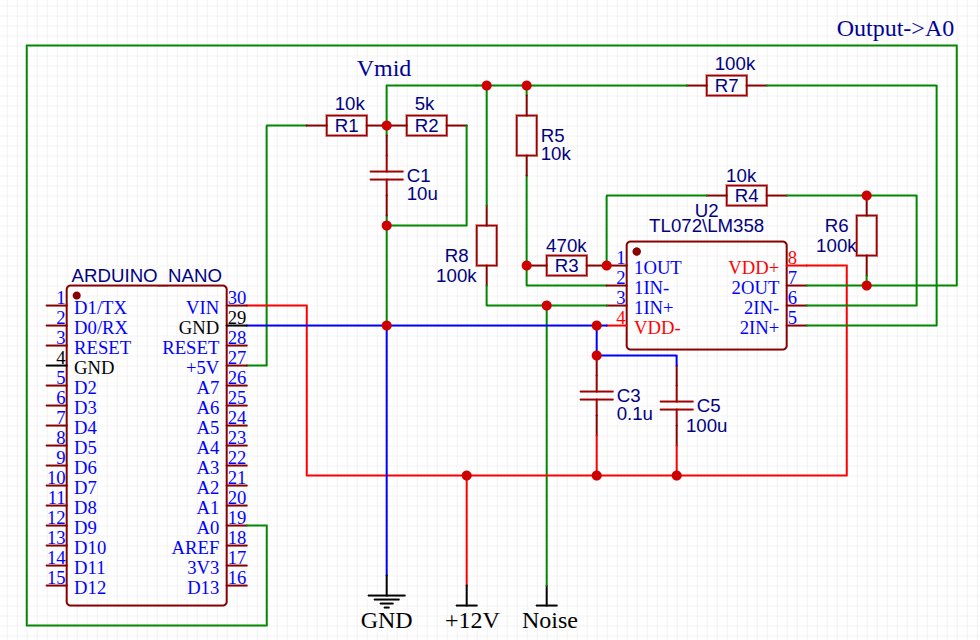
\includegraphics[width=0.78\linewidth,keepaspectratio]{amplifier_schemas/amp_2stage.png}
  \par\vspace{0.4em}
  \small Двухкаскадный неинвертирующий ($G\approx 528$), $+12$\,В однополярно;
  $V_\mathrm{mid}$ --- от шины $+5$\,В Arduino через делитель.
\end{frame}

% ============================================================
\begin{frame}{Канал BJT --- лавинный пробой BE-перехода}
  \begin{columns}[c]
    \begin{column}{0.48\linewidth}
      \centering
      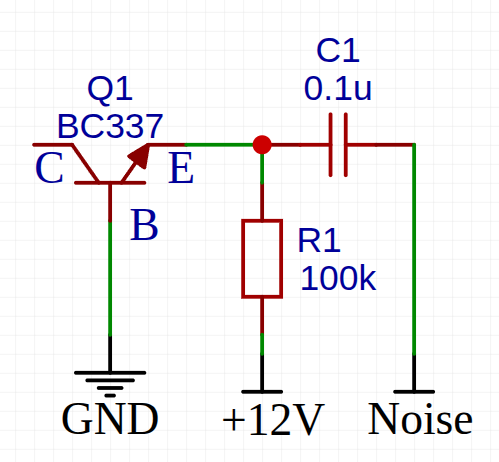
\includegraphics[width=\linewidth,keepaspectratio]{bjt_noise_source/schema.png}
    \end{column}
    \begin{column}{0.48\linewidth}
      \footnotesize
      Q1 = BC337 включён инвертированно:
      \begin{itemize}\setlength{\itemsep}{0.2em}
        \item C, B --- на землю;
        \item E через $R_b{=}100$\,кОм $\to$ $+12$\,В;
        \item $U_{BR}\sim 7\ldots 9$\,В.
      \end{itemize}
      \vspace{0.3em}
      Снятие сигнала: через $C_1{=}0{,}1$\,мкФ на вход усилителя.
    \end{column}
  \end{columns}
\end{frame}

% ============================================================
\begin{frame}{Эволюция канала BJT}
  \begin{columns}[c]
    \begin{column}{0.55\linewidth}
      \footnotesize
      \begin{tabular}{|c|p{0.50\linewidth}|c|c|}
        \hline
        \textbf{Эт.} & \textbf{Конфигурация} & $\sigma_\mathrm{adc}$ & \textbf{NIST} \\
        \hline
        1 & 1 каскад, $G\!\approx\!48$ & $28$ & 12/3 \\
        \hline
        2 & 2 каскада, $G\!\approx\!528$ & $145$ & 13/2$^\ast$ \\
        \hline
        3 & коррекция $V_\mathrm{mid}\!\downarrow$ & $122$ & 12/3 \\
        \hline
        \textbf{4} & \textbf{развязка питания} & $\mathbf{146}$ & \textbf{13/2} \\
        \hline
      \end{tabular}
      \par\vspace{0.3em}
      \tiny$^\ast$за счёт насыщения АЦП.
    \end{column}
    \begin{column}{0.42\linewidth}
      \centering
      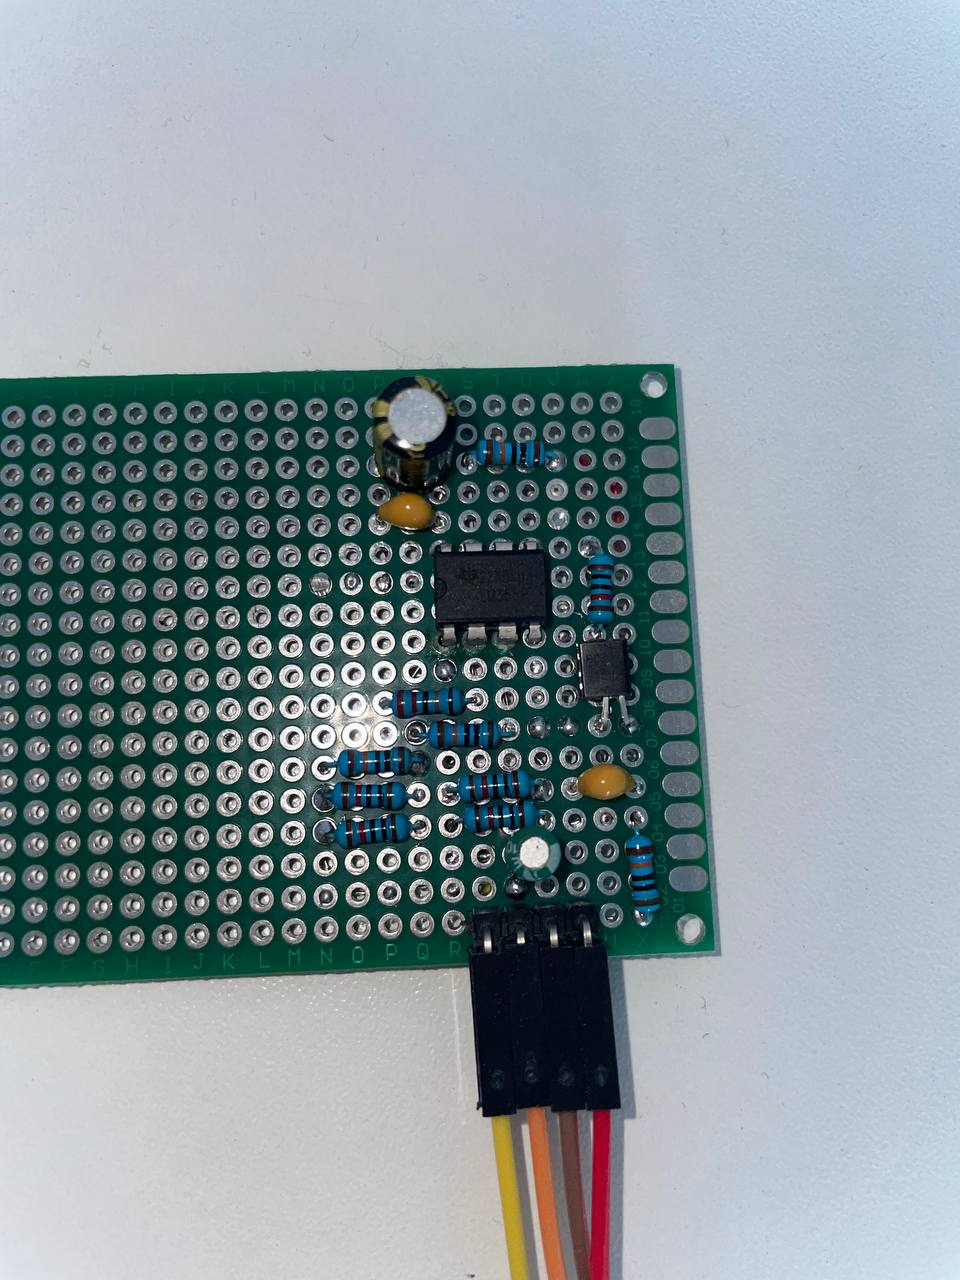
\includegraphics[width=0.88\linewidth,keepaspectratio]{photo_trng_bjt_module/board.jpg}
    \end{column}
  \end{columns}
\end{frame}

% ============================================================
\begin{frame}{Постобработка битового потока}
  \begin{columns}[T]
    \begin{column}{0.48\linewidth}
      \textbf{Фон Нейман} (база)
      \par\vspace{0.4em}
      $(0,1)\!\to\! 0,\quad (1,0)\!\to\! 1$\\
      $(0,0),(1,1)\!\to\!$ отброс
      \par\vspace{0.4em}
      \small некриптографический,\\ диагностичный экстрактор
    \end{column}
    \begin{column}{0.48\linewidth}
      \textbf{Каскад} (этап\,4)
      \par\vspace{0.4em}
      VN $\to$ \texttt{decim\_xor8win}
      \par\vspace{0.4em}
      \small 8 подряд бит выхода VN\\$\to$ XOR $\to$ 1 бит
    \end{column}
  \end{columns}
  \vspace{0.6em}
  \centering\small\emph{SHA-256 не используется: маскирует дефекты источника.}
\end{frame}

% ============================================================
\begin{frame}{Главный результат}
  \begin{columns}[c]
    \begin{column}{0.55\linewidth}
      \centering
      \begin{minipage}{0.92\linewidth}\centering
        \fcolorbox{accent}{white}{\parbox{0.94\linewidth}{\centering\Large
        \vspace{0.4em}\textbf{\color{accent} NIST STS}\par
        \vspace{0.3em}{\Huge\bfseries 15 / 15}\par
        \vspace{0.1em}{\normalsize PASS / FAIL\,=\,0\,/\,N/A\,=\,0}\par\vspace{0.4em}}}
      \end{minipage}
      \par\vspace{0.6em}
      \footnotesize
      Канал BJT, этап 4 $+$ каскад VN\,$\to$\,\texttt{decim\_xor8win}\\
      min-H\,=\,0{,}9999 бит/бит;
      $\sim 1{,}6$\,кбит/с;\\
      элементная база $<$\,50\,руб.
    \end{column}
    \begin{column}{0.43\linewidth}
      \centering
      
\includegraphics[width=0.85\linewidth,keepaspectratio]{exp_bjt_aftervn/bits_image.png}
      \par\vspace{0.2em}{\tiny битовый поток $512\times512$ после каскада}
    \end{column}
  \end{columns}
\end{frame}

% ============================================================
\begin{frame}{Сравнение источников}
  \centering
  \scriptsize
  \setlength{\tabcolsep}{3pt}
  \renewcommand{\arraystretch}{1.1}
  \begin{tabular}{|p{0.30\linewidth}|c|c|c|c|}
    \hline
    \textbf{Канал} & $\sigma_\mathrm{adc}$ & \textbf{NIST} & \textbf{min-H} & \textbf{бит/с} \\
    \hline
    \textbf{BJT + VN + XOR-каскад} & $147$ & \textbf{15 / 0} & $0{,}9999$ & ${\sim}\,1{,}6{\cdot}10^3$ \\
    \hline
    BJT + VN (базовый) & $147$ & 13 / 2 & $0{,}9999$ & ${\sim}\,1{,}3{\cdot}10^4$ \\
    \hline
    Тепловой шум $10$\,МОм & $15$ & 10 / 5 & $0{,}9984$ & ${\sim}\,1{,}5{\cdot}10^4$ \\
    \hline
    Микрофон KY-037 & $1$ & 4 / 11 & $0{,}9994$ & ${\sim}\,7{,}5{\cdot}10^3$ \\
    \hline
    MPU-6050 (MEMS) & --- & 2 / 11 & $0{,}584$ & ${\sim}\,5{,}6{\cdot}10^3$ \\
    \hline
    Плавающий АЦП / clock jitter & --- & 0 / 15 & --- & ${\sim}\,10^2$ \\
    \hline
  \end{tabular}
\end{frame}

% ============================================================
\begin{frame}{Выводы}
  \begin{itemize}
    \setlength{\itemsep}{0.7em}
    \item Сконструирован стенд, проверены $6$ независимых источников энтропии.
    \item Лучший результат --- \textbf{BJT $+$ каскадная постобработка: 15/15 NIST STS}.
    \item Двухступенчатая некриптографическая постобработка \emph{эквивалентна} криптографическому отбеливанию по эффекту на NIST.
    \item Стоимость элементной базы канала $<$\,$50$\,руб.
  \end{itemize}
\end{frame}

% ============================================================
\begin{frame}{Перспективы}
  \begin{itemize}
    \setlength{\itemsep}{0.7em}
    \item Второй идентичный канал на втором ОУ корпуса $+$ XOR-смешение.
    \item Печатная плата с экранированием и низкошумящим LDO для ОУ.
    \item Упаковка в законченный модуль с собственным микроконтроллером.
  \end{itemize}
\end{frame}

% ============================================================
\begin{frame}[plain]
  \centering
  \vfill
  {\Huge\bfseries\color{accent} Спасибо за внимание!\par}
  \vspace{1em}
  {\large Готов ответить на вопросы.}
  \vfill
\end{frame}

\end{document}
